\documentclass[11pt,a4paper]{article}

% Paquetes
\usepackage[utf8]{inputenc}
\usepackage[T1]{fontenc}
\usepackage[spanish]{babel}
\usepackage[margin=2.5cm]{geometry}
\usepackage{graphicx}
\usepackage{xcolor}
\usepackage{colortbl}
\usepackage{booktabs}
\usepackage{longtable}
\usepackage{array}
\usepackage{enumitem}
\usepackage{titlesec}
\usepackage{fancyhdr}
\usepackage{tcolorbox}
\usepackage{hyperref}
\usepackage{listings}

% Colores
\definecolor{primary}{HTML}{2563EB}
\definecolor{critical}{HTML}{DC2626}
\definecolor{success}{HTML}{10B981}
\definecolor{warning}{HTML}{F59E0B}
\definecolor{codebg}{HTML}{F1F5F9}
\definecolor{codeframe}{HTML}{CBD5E1}

% Hyperlinks
\hypersetup{
    colorlinks=true,
    linkcolor=primary,
    urlcolor=primary,
    citecolor=primary,
    pdftitle={Resiliencia y LLM - Sentinel AcademIA},
    pdfauthor={Equipo Sentinel AcademIA}
}

% Listings (codigo TypeScript - definicion personalizada)
\lstdefinelanguage{TypeScript}{
  keywords={async, await, interface, type, enum, const, let, var, function, return, if, else, for, while, try, catch, throw, new, import, from, export, default, class, extends, implements, public, private, protected, static, readonly, void, null, undefined, true, false, this, super, in, of, instanceof, typeof, as, satisfies},
  keywordstyle=\color{primary}\bfseries,
  ndkeywords={string, number, boolean, any, unknown, never, object, Promise, Array, Record, Partial, Required, Readonly},
  ndkeywordstyle=\color{warning}\bfseries,
  sensitive=true,
  comment=[l]{//},
  morecomment=[s]{/*}{*/},
  commentstyle=\color{gray}\itshape,
  stringstyle=\color{success},
  morestring=[b]',
  morestring=[b]"
}

\lstdefinelanguage{YAML}{
  keywords={true, false, null, yes, no},
  keywordstyle=\color{primary}\bfseries,
  sensitive=true,
  comment=[l]{\#},
  commentstyle=\color{gray}\itshape,
  stringstyle=\color{success},
  morestring=[b]",
  morestring=[b]'
}

\lstdefinelanguage{SQL}{
  keywords={SELECT, FROM, WHERE, AND, OR, NOT, NULL, AS, BY, ORDER, GROUP, HAVING, LIMIT, COUNT, SUM, AVG, MIN, MAX, DESC, ASC, DISTINCT, IN, LIKE, BETWEEN, EXISTS, JOIN, LEFT, RIGHT, INNER, OUTER, ON, STATS, FIELDS, FILTER, SORT, BIN, PERCENTILE},
  keywordstyle=\color{primary}\bfseries,
  ndkeywords={fields, filter, stats, sort, bin, percentile, count, sum, avg, min, max, limit},
  ndkeywordstyle=\color{warning}\bfseries,
  sensitive=false,
  comment=[l]{//},
  commentstyle=\color{gray}\itshape,
  stringstyle=\color{success},
  morestring=[b]',
  morestring=[b]"
}

\lstset{
    basicstyle=\ttfamily\small,
    backgroundcolor=\color{codebg},
    frame=single,
    framerule=0.5pt,
    rulecolor=\color{codeframe},
    breaklines=true,
    showstringspaces=false,
    numbers=left,
    numberstyle=\tiny\color{gray},
    numbersep=8pt,
    stringstyle=\color{success},
}

% Formato titulos
\titleformat{\section}{\Large\bfseries\color{primary}}{\thesection}{1em}{}
\titleformat{\subsection}{\large\bfseries\color{primary!80!black}}{\thesubsection}{1em}{}
\titleformat{\subsubsection}{\normalsize\bfseries\color{primary!70!black}}{\thesubsubsection}{1em}{}

% Header/footer
\pagestyle{fancy}
\fancyhf{}
\rhead{\small Sentinel AcademIA \textbar{} Criterio 3}
\lhead{\small Resiliencia y LLM}
\rfoot{\thepage}
\renewcommand{\headrulewidth}{0.4pt}

% Title
\title{
    \vspace{-1cm}
    {\Huge\bfseries\color{primary} Resiliencia, Manejo de L\'imites y LLM}\\[0.4cm]
    {\Large Estrategias de robustez en Sentinel AcademIA}\\[0.6cm]
    {\normalsize Circuit Breaker, Fallback, Rate Limiting, DLQ, Idempotencia y Observabilidad}
}
\author{
    \textbf{Equipo de Desarrollo} \\
    \texttt{sentinel-academia@universidad.edu}
}
\date{\today}

\begin{document}

\maketitle
\thispagestyle{fancy}

\begin{tcolorbox}[colback=codebg, colframe=primary, title=\textbf{Resumen Ejecutivo}]
\small
Este documento detalla las \textbf{9 estrategias de resiliencia} implementadas en Sentinel AcademIA para garantizar la robustez del sistema ante fallos de la IA generativa, picos de carga, errores externos y problemas de red. La arquitectura est\'a dise\~nada para \textbf{degradar de forma elegante} (de Cohere Command R $\rightarrow$ Llama 3.1 $\rightarrow$ Command R+ $\rightarrow$ respuesta controlada), mantener \textbf{idempotencia exactly-once} en consumers SQS, y proporcionar \textbf{observabilidad end-to-end} con CloudWatch, X-Ray y Langfuse. El sistema cumple SLA objetivo de \textbf{99\% de \'exito en procesamiento} y \textbf{detecci\'on de casos cr\'iticos en $<$ 1 minuto}.
\end{tcolorbox}

\tableofcontents
\newpage

% ============================================
\section{Introducci\'on: Por qu\'e la resiliencia es cr\'itica}
% ============================================

Sentinel AcademIA depende de m\'ultiples servicios externos y distribuidos:

\begin{itemize}[leftmargin=*]
    \item \textbf{Oracle OCI Generative AI}: provee el LLM, puede tener rate limits o ca\'idas
    \item \textbf{AWS SQS / DynamoDB / S3}: servicios managed pero no 100\% disponibles
    \item \textbf{Red cross-region}: latencia variable entre AWS y OCI ($\sim$80ms)
    \item \textbf{Frontend Vercel}: deploy en edge, posibles problemas de cache
\end{itemize}

Sin estrategias de resiliencia, una ca\'ida de OCI GenAI de 5 minutos significar\'ia perder el an\'alisis de cientos de quejas, incluyendo las cr\'iticas. \textbf{Esto es inaceptable} para un sistema que detecta casos de salud mental o acoso.

\subsection{Las 9 estrategias implementadas}

\begin{enumerate}[leftmargin=*]
    \item \textbf{Timeouts} en TODA llamada externa
    \item \textbf{Circuit Breaker} con opossum
    \item \textbf{Fallback chain} entre 3 modelos LLM
    \item \textbf{Rate limiting} con token bucket
    \item \textbf{Retry} con exponential backoff y jitter
    \item \textbf{Idempotencia} con SHA-256 y conditional writes
    \item \textbf{Dead Letter Queues} en cada cola SQS
    \item \textbf{Validaci\'on Zod} del output del LLM
    \item \textbf{Observabilidad} con CloudWatch, X-Ray, Langfuse
\end{enumerate}

\begin{tcolorbox}[colback=red!5!white, colframe=critical, title=\textbf{Principio fundamental}]
\textit{``Dise\~nar para el fallo, no para el camino feliz.''} Toda llamada externa PUEDE fallar. Toda respuesta PUEDE llegar mal. Todo servicio PUEDE caerse. El sistema debe seguir operando de forma degradada.
\end{tcolorbox}

% ============================================
\section{Timeouts en Llamadas Externas}
% ============================================

\subsection{Configuraci\'on est\'andar}

Toda llamada a un servicio externo tiene un timeout expl\'icito. \textbf{Nunca} se usa el default del SDK (que puede ser de minutos o inexistente).

\begin{lstlisting}[language=TypeScript, caption={Timeout en AWS SDK v3}, label={lst:aws-timeout}]
import { DynamoDBClient } from '@aws-sdk/client-dynamodb';
import { S3Client } from '@aws-sdk/client-s3';

const dynamoClient = new DynamoDBClient({
  region: process.env.AWS_REGION,
  requestHandler: {
    requestTimeout: 5_000,    // 5 segundos para DynamoDB
    connectionTimeout: 2_000,  // 2 segundos para TCP handshake
  },
});

const s3Client = new S3Client({
  region: process.env.AWS_REGION,
  requestHandler: {
    requestTimeout: 10_000,   // 10 segundos para S3
    connectionTimeout: 3_000,
  },
});
\end{lstlisting}

\begin{lstlisting}[language=TypeScript, caption={Timeout en OCI SDK}]
import { GenerativeAiInferenceClient } from 'oci-generativeaiinference';

const genaiClient = new GenerativeAiInferenceClient({
  authenticationDetailsProvider: new DefaultConfigAuthenticationDetailsProvider(),
  region: process.env.OCI_REGION ?? 'us-chicago-1',
});
// Timeout via AbortController
const controller = new AbortController();
const timeoutId = setTimeout(() => controller.abort(), 30_000);

try {
  const response = await genaiClient.generateText(
    { generateTextDetails },
    { abortSignal: controller.signal }
  );
} finally {
  clearTimeout(timeoutId);
}
\end{lstlisting}

\subsection{Timeouts por servicio}

\begin{longtable}{|p{4cm}|p{3cm}|p{2.5cm}|p{4cm}|}
\hline
\rowcolor{primary!20}
\textbf{Servicio} & \textbf{Operaci\'on} & \textbf{Timeout} & \textbf{Justificaci\'on} \\
\hline
\endhead
DynamoDB & GetItem, PutItem, Query & 5s & Operaci\'on simple, debe ser r\'apida \\
\hline
S3 & GetObject, PutObject & 10s & Puede ser archivo grande \\
\hline
SQS & SendMessage, ReceiveMessage & 10s & Confiable pero no instant\'aneo \\
\hline
EventBridge & PutEvents & 5s & Operaci\'on simple \\
\hline
SNS & Publish & 10s & Confiable \\
\hline
OCI GenAI & generateText & 30s & LLM puede tardar en razonar \\
\hline
OCI Document AI & analyzeDocument & 60s & PDFs grandes tardan m\'as \\
\hline
SES (email) & SendEmail & 10s & Confiable \\
\hline
\end{longtable}

% ============================================
\section{Circuit Breaker con opossum}
% ============================================

\subsection{Qu\'e es y por qu\'e lo necesitamos}

Un circuit breaker es un patr\'on que previene llamadas a un servicio que est\'a fallando. Funciona como un interruptor el\'ectrico:

\begin{itemize}[leftmargin=*]
    \item \textbf{CLOSED} (cerrado): llamadas pasan normalmente
    \item \textbf{OPEN} (abierto): llamadas se rechazan inmediatamente (fail-fast)
    \item \textbf{HALF\_OPEN}: tras un tiempo, se permite UNA llamada de prueba
\end{itemize}

Si OCI GenAI empieza a fallar (50\% de errores), \textbf{no queremos seguir gastando tiempo y dinero} en llamadas que van a fallar. El circuit breaker las rechaza al instante, permiti\'endonos caer al siguiente modelo de la cadena de fallback.

\subsection{Implementaci\'on con opossum}

\begin{lstlisting}[language=TypeScript, caption={Circuit breaker para Cohere Command R}]
import CircuitBreaker from 'opossum';
import { ociGenai } from './ociGenai';
import { logger } from '../handlers/_shared/logger';

interface GenerateArgs {
  prompt: string;
  systemPrompt?: string;
  maxTokens?: number;
  temperature?: number;
}

async function callCohere(args: GenerateArgs): Promise<string> {
  return ociGenai.generateText(args.prompt, {
    model: 'cohere.command-r',
    systemPrompt: args.systemPrompt,
    maxTokens: args.maxTokens,
    temperature: args.temperature,
  });
}

const breaker = new CircuitBreaker(callCohere, {
  timeout: 30_000,              // 30 segundos max por llamada
  errorThresholdPercentage: 50, // 50% de errores -> abre
  resetTimeout: 30_000,         // 30 segundos en estado OPEN antes de probar
  rollingCountTimeout: 10_000,  // Ventana de 10s para calcular %
  rollingCountBuckets: 10,      // 10 buckets en la ventana
  volumeThreshold: 5,           // Minimo 5 calls antes de evaluar
  name: 'cohere-command-r',
});

// Eventos para observabilidad
breaker.on('open', () => logger.warn('Circuit OPEN - OCI Cohere', { breaker: 'cohere' }));
breaker.on('halfOpen', () => logger.info('Circuit HALF_OPEN - probando OCI Cohere'));
breaker.on('close', () => logger.info('Circuit CLOSED - OCI Cohere recuperado'));
breaker.on('reject', () => logger.warn('Call rechazada por circuit abierto'));
breaker.on('timeout', () => logger.error('Timeout en OCI Cohere'));
breaker.on('failure', (err) => logger.error('Fallo en OCI Cohere', { error: String(err) }));

export async function callCohereSafe(args: GenerateArgs): Promise<string> {
  return breaker.fire(args);
}
\end{lstlisting}

\subsection{M\'etricas del circuit breaker}

\begin{lstlisting}[language=TypeScript, caption={Exponer metricas del circuit breaker}]
// En CloudWatch custom metrics
import { CloudWatch } from '@aws-sdk/client-cloudwatch';

setInterval(() => {
  const cw = new CloudWatch({});
  cw.putMetricData({
    Namespace: 'SentinelAcademia/CircuitBreaker',
    MetricData: [
      {
        MetricName: 'State',
        Value: breaker.opened ? 1 : 0,
        Unit: 'None',
        Dimensions: [{ Name: 'Breaker', Value: 'cohere-command-r' }],
      },
      {
        MetricName: 'Failures',
        Value: breaker.stats.failures,
        Unit: 'Count',
        Dimensions: [{ Name: 'Breaker', Value: 'cohere-command-r' }],
      },
      {
        MetricName: 'Successes',
        Value: breaker.stats.successes,
        Unit: 'Count',
        Dimensions: [{ Name: 'Breaker', Value: 'cohere-command-r' }],
      },
    ],
  });
}, 60_000);  // Cada 60 segundos
\end{lstlisting}

% ============================================
\section{Fallback Chain Multi-Modelo}
% ============================================

\subsection{Cadena de modelos}

El sistema intenta los modelos en orden de \textbf{costo-beneficio}:

\begin{enumerate}[leftmargin=*]
    \item \textbf{Cohere Command R} (primario): \$0.50 input / \$1.50 output por 1M tokens
    \item \textbf{Llama 3.1 70B} (secundario): \$0.72 input / \$0.72 output por 1M tokens
    \item \textbf{Cohere Command R+} (terciario): \$3.00 input / \$15.00 output por 1M tokens
    \item \textbf{Respuesta controlada} (degradado): mensaje fijo sin LLM
\end{enumerate}

\begin{tcolorbox}[colback=success!10!white, colframe=success, title=\textbf{Decisi\'on de costos}]
Usar Command R+ como terciario (no primario) reduce costos en $\sim$70\% vs. una arquitectura que lo usara siempre, mientras mantiene calidad cuando los modelos baratos fallan.
\end{tcolorbox}

\subsection{Implementaci\'on del router con fallback}

\begin{lstlisting}[language=TypeScript, caption={LLM Router con fallback chain}]
import { callCohereSafe } from './breakers/cohereBreaker';
import { callLlamaSafe } from './breakers/llamaBreaker';
import { callCommandPlusSafe } from './breakers/commandPlusBreaker';
import { logger } from '../handlers/_shared/logger';

export interface GenerateArgs {
  prompt: string;
  systemPrompt?: string;
  maxTokens?: number;
  temperature?: number;
}

export async function generateWithFallback(args: GenerateArgs): Promise<string> {
  const models = [
    { name: 'cohere.command-r', fn: () => callCohereSafe(args) },
    { name: 'meta.llama-3.1-70b-instruct', fn: () => callLlamaSafe(args) },
    { name: 'cohere.command-r-plus', fn: () => callCommandPlusSafe(args) },
  ];

  for (const model of models) {
    try {
      const result = await model.fn();
      logger.info('LLM call exitosa', { model: model.name, length: result.length });
      return result;
    } catch (err) {
      logger.error('LLM call fallo, intentando siguiente', {
        model: model.name,
        error: String(err),
      });
      // Continuar al siguiente modelo
    }
  }

  // Todos los modelos fallaron: respuesta controlada
  logger.error('Todos los modelos LLM fallaron, usando respuesta controlada');
  return safeDefaultResponse();
}

function safeDefaultResponse(): string {
  return JSON.stringify({
    categoria: 'OTRA',
    subcategoria: 'NO_CLASIFICADA',
    criticidad: 'MEDIA',
    criticidadJustificacion: 'Sistema no disponible para clasificar automaticamente. Requiere revision manual.',
    sentimiento: 'NEUTRO',
    entidades: [],
    temasClave: [],
    accionSugerida: 'Revision manual por equipo de bienestar',
    prioridad: 5,
    requiereNotificacionInmediata: false,
    metadata: {
      analisisFallback: true,
      timestamp: new Date().toISOString(),
    },
  });
}
\end{lstlisting}

\subsection{Justificaci\'on de cada modelo}

\begin{longtable}{|p{4cm}|p{2.5cm}|p{2.5cm}|p{4.5cm}|}
\hline
\rowcolor{primary!20}
\textbf{Modelo} & \textbf{Costo/1M in} & \textbf{Costo/1M out} & \textbf{Cu\'ando usarlo} \\
\hline
\endhead
cohere.command-r & \$0.50 & \$1.50 & \textbf{Primary}. Excelente en JSON/structured output, barato, r\'apido. Suficiente para $>$80\% de los casos. \\
\hline
meta.llama-3.1-70b-instruct & \$0.72 & \$0.72 & \textbf{Fallback 1}. Open weights, robusto, mismo precio input/output. Bueno para chat y RAG. \\
\hline
cohere.command-r-plus & \$3.00 & \$15.00 & \textbf{Fallback 2}. Reservado para casos extremos. 5x m\'as caro que R. Razonamiento profundo. \\
\hline
Respuesta controlada & \$0 & \$0 & \textbf{Degradado}. Garantiza que el sistema NUNCA falla por el LLM. Marca para revisi\'on manual. \\
\hline
\end{longtable}

% ============================================
\section{Rate Limiting con Token Bucket}
% ============================================

\subsection{Algoritmo y justificaci\'on}

Implementamos \textbf{token bucket} mediante la librer\'ia \texttt{rate-limiter-flexible}. Cada usuario tiene una "balde" que se rellena con tokens a velocidad constante. Cada request consume un token. Si no hay tokens, se rechaza con HTTP 429.

\begin{lstlisting}[language=TypeScript, caption={Rate limiter por usuario y por IP}]
import { RateLimiterMemory, RateLimiterRedis } from 'rate-limiter-flexible';

// En memoria (hackathon) o Redis (produccion)
const userLimiter = new RateLimiterMemory({
  points: 100,        // 100 requests
  duration: 60,       // por 60 segundos
  blockDuration: 60,  // bloqueo 60s si se excede
});

const ipLimiter = new RateLimiterMemory({
  points: 200,        // 200 requests
  duration: 60,       // por minuto
});

export async function checkRateLimit(userId: string, ip: string): Promise<{
  allowed: boolean;
  retryAfter?: number;
}> {
  try {
    await userLimiter.consume(userId, 1);
    await ipLimiter.consume(ip, 1);
    return { allowed: true };
  } catch (err) {
    if (err instanceof Error) {
      return { allowed: false, retryAfter: 60 };
    }
    return { allowed: false };
  }
}
\end{lstlisting}

\subsection{Integraci\'on en handler}

\begin{lstlisting}[language=TypeScript, caption={Rate limit en Lambda API Gateway}]
import { checkRateLimit } from './_shared/rateLimiter';

export const handler = withErrorHandling(async (event) => {
  const userId = event.requestContext.authorizer?.jwt?.claims?.sub ?? 'anonymous';
  const ip = event.requestContext.http?.sourceIp ?? '0.0.0.0';

  const rate = await checkRateLimit(userId, ip);
  if (!rate.allowed) {
    return {
      statusCode: 429,
      headers: {
        'Retry-After': String(rate.retryAfter),
        'x-correlation-id': getCorrelationId(event),
      },
      body: JSON.stringify({
        code: 'RATE_LIMITED',
        message: 'Demasiadas solicitudes. Intenta en 60 segundos.',
        correlationId: getCorrelationId(event),
      }),
    };
  }

  // Continuar con la logica normal...
});
\end{lstlisting}

\subsection{Configuraci\'on por endpoint}

\begin{longtable}{|p{5cm}|p{4cm}|p{4cm}|}
\hline
\rowcolor{primary!20}
\textbf{Endpoint} & \textbf{L\'imite} & \textbf{Raz\'on} \\
\hline
\endhead
POST /api/quejas & 5/min por usuario & Evita spam de quejas duplicadas \\
\hline
GET /api/quejas & 60/min por usuario & Lectura es barata \\
\hline
POST /api/chat & 20/min por usuario & LLM es caro \\
\hline
GET /api/dashboard/metrics & 30/min por usuario & Cache deberia estar activo \\
\hline
\end{longtable}

% ============================================
\section{Retry con Exponential Backoff y Jitter}
% ============================================

\subsection{Cu\'ando reintentar}

\textbf{S\'i reintentar}:
\begin{itemize}[leftmargin=*]
    \item Errores de red transitorios (5xx, ECONNRESET, ETIMEDOUT)
    \item Rate limits (429) con Retry-After
    \item Timeouts (superados pero no cr\'iticos)
\end{itemize}

\textbf{NO reintentar}:
\begin{itemize}[leftmargin=*]
    \item Errores 4xx del cliente (validacion, auth)
    \item Errores de programacion (TypeError, etc)
    \item Despu\'es de 3 intentos
\end{itemize}

\subsection{Implementaci\'on con p-retry}

\begin{lstlisting}[language=TypeScript, caption={Retry con exponential backoff}]
import pRetry, { AbortError } from 'p-retry';

async function callWithRetry<T>(
  fn: () => Promise<T>,
  options: { retries?: number; minTimeout?: number; maxTimeout?: number } = {}
): Promise<T> {
  return pRetry(fn, {
    retries: options.retries ?? 3,
    minTimeout: options.minTimeout ?? 1000,    // 1 segundo
    maxTimeout: options.maxTimeout ?? 10_000,  // 10 segundos
    factor: 2,                                  // Backoff exponencial
    randomize: true,                            // Jitter
    onFailedAttempt: (error) => {
      logger.warn('Reintento', {
        attempt: error.attemptNumber,
        retriesLeft: error.retriesLeft,
        error: String(error),
      });
    },
  });
}

// Uso
const result = await callWithRetry(() => callCohereSafe(args), { retries: 3 });
\end{lstlisting}

\subsection{Backoff exponencial + jitter}

El jitter evita "thundering herd" (todos reintentan al mismo tiempo):

\begin{lstlisting}[language=TypeScript, caption={Calculo del delay con jitter}]
function calculateDelay(attempt: number, baseMs: number = 1000): number {
  // Exponential: 1s, 2s, 4s, 8s, 16s
  const exponential = baseMs * Math.pow(2, attempt);
  // Cap at 30 seconds
  const capped = Math.min(exponential, 30_000);
  // Jitter: +/- 25% del valor
  const jitter = capped * (0.75 + Math.random() * 0.5);
  return Math.floor(jitter);
}

// Ejemplo de delays: 750ms, 2200ms, 3100ms, 8500ms
\end{lstlisting}

% ============================================
\section{Idempotencia Exactly-Once Processing}
% ============================================

\subsection{El problema}

SQS garantiza \textbf{at-least-once delivery}: un mensaje puede entregarse m\'as de una vez. Si nuestra Lambda processQueja procesa el mismo mensaje 2 veces, el LLM se llama 2 veces (gastamos dinero) y se duplica el an\'alisis en DynamoDB.

\subsection{La soluci\'on: SHA-256 + conditional writes}

\begin{lstlisting}[language=TypeScript, caption={Idempotencia con hash y conditional writes}]
import { createHash } from 'crypto';
import { docClient, TABLE_NAME } from '../handlers/_shared/dynamoClient';
import { PutCommand } from '@aws-sdk/lib-dynamodb';

function computeIdempotencyKey(payload: unknown): string {
  // Normalizar y hashear
  const normalized = JSON.stringify(payload, Object.keys(payload as object).sort());
  return createHash('sha256').update(normalized).digest('hex');
}

async function processQueja(message: QuejaProcessMessage): Promise<void> {
  const idempotencyKey = computeIdempotencyKey(message.payload);

  // 1. Check si ya fue procesada
  const existing = await docClient.send(new GetCommand({
    TableName: TABLE_NAME,
    Key: { pk: `IDEMPOTENCY#${idempotencyKey}`, sk: 'PROCESSED' },
  }));

  if (existing.Item) {
    logger.info('Queja ya procesada, saltando', { idempotencyKey });
    return;  // ACK del mensaje
  }

  // 2. Procesar la queja con el LLM
  const analysis = await analizarQueja(message.payload.input);

  // 3. Transaccion atomica: guardar analisis + marcar como procesada
  await docClient.send(new TransactWriteCommand({
    TransactItems: [
      {
        Put: {
          TableName: TABLE_NAME,
          Item: {
            pk: `QUEJA#${message.payload.quejaId}`,
            sk: 'ANALYSIS#' + new Date().toISOString(),
            ...analysis,
            quejaId: message.payload.quejaId,
            createdAt: new Date().toISOString(),
          },
        },
      },
      {
        Put: {
          TableName: TABLE_NAME,
          Item: {
            pk: `IDEMPOTENCY#${idempotencyKey}`,
            sk: 'PROCESSED',
            quejaId: message.payload.quejaId,
            processedAt: new Date().toISOString(),
            ttl: Math.floor(Date.now() / 1000) + (7 * 24 * 60 * 60),  // 7 dias
          },
          ConditionExpression: 'attribute_not_exists(pk)',  // Atomic check
        },
      },
    ],
  }));

  logger.info('Queja procesada exitosamente', { quejaId: message.payload.quejaId });
}
\end{lstlisting}

% ============================================
\section{Dead Letter Queues (DLQ)}
% ============================================

\subsection{Obligatorias en cada cola}

Toda cola SQS tiene una DLQ asociada. Despu\'es de 3 intentos fallidos, el mensaje va a la DLQ para inspecci\'on manual.

\begin{lstlisting}[language=TypeScript, caption={Report batch item failures}]
import { SQSEvent, SQSBatchResponse } from 'aws-lambda';

export const handler = async (event: SQSEvent): Promise<SQSBatchResponse> => {
  const failures: { itemIdentifier: string }[] = [];

  for (const record of event.Records) {
    try {
      const message = JSON.parse(record.body) as QuejaProcessMessage;
      await processQueja(message);
    } catch (err) {
      logger.error('Error procesando mensaje', {
        messageId: record.messageId,
        error: String(err),
      });
      failures.push({ itemIdentifier: record.messageId });
    }
  }

  return { batchItemFailures: failures };
};
\end{lstlisting}

\subsection{SAM template para DLQ}

\begin{lstlisting}[language=YAML, caption={SAM: SQS con DLQ obligatoria}]
ComplaintsQueue:
  Type: AWS::SQS::Queue
  Properties:
    QueueName: complaints-queue
    VisibilityTimeout: 180       # 6x el timeout de la Lambda
    MessageRetentionPeriod: 1209600  # 14 dias
    RedrivePolicy:
      deadLetterTargetArn: !GetAtt ComplaintsDLQ.Arn
      maxReceiveCount: 3

ComplaintsDLQ:
  Type: AWS::SQS::Queue
  Properties:
    QueueName: complaints-dlq
    MessageRetentionPeriod: 1209600

# Alarma si la DLQ tiene mensajes
DLQAlarm:
  Type: AWS::CloudWatch::Alarm
  Properties:
    AlarmName: complaints-dlq-not-empty
    MetricName: ApproximateNumberOfMessagesVisible
    Namespace: AWS/SQS
    Dimensions:
      - Name: QueueName
        Value: !GetAtt ComplaintsDLQ.QueueName
    Statistic: Sum
    Period: 300
    EvaluationPeriods: 1
    Threshold: 0
    ComparisonOperator: GreaterThanThreshold
    AlarmActions:
      - !Ref AlertTopic
\end{lstlisting}

% ============================================
\section{Validaci\'on del Output del LLM con Zod}
% ============================================

\subsection{El problema de los LLMs}

Los LLMs no siempre devuelven JSON v\'alido. A veces:
\begin{itemize}[leftmargin=*]
    \item Agregan markdown de tipo ``triple backtick json'' alrededor del JSON
    \item Incluyen explicaciones antes/despu\'es
    \item Inventan campos extra
    \item Omiten campos requeridos
    \item Devuelven strings en campos que deber\'ian ser n\'umeros
\end{itemize}

\subsection{Schema Zod estricto}

\begin{lstlisting}[language=TypeScript, caption={Schema Zod para validacion}]
import { z } from 'zod';

export const AnalisisSchema = z.object({
  categoria: z.enum([
    'ACADEMICA', 'INFRAESTRUCTURA', 'ACOSO',
    'ADMINISTRATIVA', 'SALUD', 'OTRA'
  ]),
  subcategoria: z.string().min(1).max(100),
  criticidad: z.enum(['BAJA', 'MEDIA', 'ALTA', 'CRITICA']),
  criticidadJustificacion: z.string().min(10).max(500),
  sentimiento: z.enum(['POSITIVO', 'NEUTRO', 'NEGATIVO', 'NEGATIVO_FUERTE']),
  entidades: z.array(z.object({
    tipo: z.string(),
    texto: z.string().max(200),
  })).max(20),
  temasClave: z.array(z.string()).min(1).max(10),
  accionSugerida: z.string().min(10).max(500),
  prioridad: z.number().int().min(1).max(10),
  requiereNotificacionInmediata: z.boolean(),
}).strict();  // Rechaza campos extra

export type Analisis = z.infer<typeof AnalisisSchema>;
\end{lstlisting}

\subsection{Funciones de extracci\'on y validaci\'on}

\begin{lstlisting}[language=TypeScript, caption={Extraer JSON del output y validar}]
function extractJson(text: string): unknown {
  // Intentar parsear directamente
  try {
    return JSON.parse(text);
  } catch {
    // Buscar bloque JSON en el texto
    const match = text.match(/\{[\s\S]*\}/);
    if (!match) {
      throw new Error('No se encontro JSON en el output del LLM');
    }
    return JSON.parse(match[0]);
  }
}

export async function analizarQueja(texto: string): Promise<Analisis> {
  const raw = await generateWithFallback({
    prompt: `Analiza esta queja: """${texto}"""`,
    systemPrompt: SYSTEM_PROMPT,
    temperature: 0.3,  // Bajo para consistencia
    maxTokens: 800,
  });

  const json = extractJson(raw);
  const parsed = AnalisisSchema.safeParse(json);

  if (!parsed.success) {
    logger.error('LLM output invalido', {
      errors: parsed.error.flatten(),
      rawOutput: raw.slice(0, 500),
    });
    throw new Error(`Output invalido: ${parsed.error.message}`);
  }

  return parsed.data;
}
\end{lstlisting}

% ============================================
\section{Logging Estructurado}
% ============================================

\subsection{Formato JSON obligatorio}

Todo log es JSON v\'alido, parseable por CloudWatch Logs Insights.

\begin{lstlisting}[language=TypeScript, caption={Logger estructurado}]
type LogLevel = 'debug' | 'info' | 'warn' | 'error';

interface LogContext {
  correlationId?: string;
  userId?: string;
  quejaId?: string;
  modelo?: string;
  tokens?: number;
  latencyMs?: number;
  [key: string]: unknown;
}

class StructuredLogger {
  log(level: LogLevel, message: string, context: LogContext = {}) {
    const entry = {
      timestamp: new Date().toISOString(),
      level: level.toUpperCase(),
      message,
      service: process.env.POWERTOOLS_SERVICE_NAME ?? 'sentinel-academia',
      ...context,
    };
    console.log(JSON.stringify(entry));
  }

  debug(message: string, context?: LogContext) { this.log('debug', message, context); }
  info(message: string, context?: LogContext) { this.log('info', message, context); }
  warn(message: string, context?: LogContext) { this.log('warn', message, context); }
  error(message: string, context?: LogContext) { this.log('error', message, context); }
}

export const logger = new StructuredLogger();
\end{lstlisting}

\subsection{Correlation ID end-to-end}

El correlationId se genera en API Gateway (o en el cliente), se pasa por headers HTTP, se incluye en mensajes SQS, y se loggea en cada paso. Permite trazabilidad completa de una queja.

\begin{lstlisting}[language=TypeScript, caption={Propagacion del correlationId}]
// En el handler
const correlationId = event.headers['x-correlation-id'] ?? crypto.randomUUID();
logger.info('Lambda invoked', { correlationId });

// En el mensaje a SQS
await sqs.send(new SendMessageCommand({
  QueueUrl: QUEUE_URL,
  MessageBody: JSON.stringify({
    payload: data,
    metadata: { correlationId, attempts: 0 },
  }),
  MessageAttributes: {
    correlationId: { DataType: 'String', StringValue: correlationId },
  },
}));

// En el consumer
const correlationId = record.messageAttributes?.correlationId?.stringValue
                    ?? JSON.parse(record.body).metadata.correlationId;
logger.info('Procesando mensaje', { correlationId });
\end{lstlisting}

% ============================================
\section{Observabilidad End-to-End}
% ============================================

\subsection{CloudWatch Logs Insights queries}

\textbf{Queries utiles para debugging}:

\begin{lstlisting}[language=SQL, caption={Errores en la ultima hora}]
fields @timestamp, level, message, correlationId, error
| filter level = "ERROR"
| stats count() as total by message
| sort total desc
| limit 20
\end{lstlisting}

\begin{lstlisting}[language=SQL, caption={Trace por correlationId especifico}]
fields @timestamp, level, message, modelo, tokens, latencyMs
| filter correlationId = "abc-123-def"
| sort @timestamp asc
\end{lstlisting}

\begin{lstlisting}[language=SQL, caption={Latencia p95 de Lambdas}]
fields @timestamp, @duration
| filter @type = "REPORT"
| stats percentile(@duration, 95) as p95 by bin(5m)
\end{lstlisting}

\begin{lstlisting}[language=SQL, caption={Costos estimados de LLM}]
fields @timestamp, modelo, tokens
| filter message = "LLM call exitosa"
| stats sum(tokens) as totalTokens by modelo
| sort totalTokens desc
\end{lstlisting}

\subsection{Langfuse para tracing del LLM}

Langfuse proporciona tracing detallado de cada llamada al LLM:

\begin{lstlisting}[language=TypeScript, caption={Tracing con Langfuse}]
import { Langfuse } from 'langfuse';

const langfuse = new Langfuse({
  publicKey: process.env.LANGFUSE_PUBLIC_KEY!,
  secretKey: process.env.LANGFUSE_SECRET_KEY!,
  baseUrl: process.env.LANGFUSE_HOST,
});

export async function generateWithFallbackTraced(args: GenerateArgs): Promise<string> {
  const trace = langfuse.trace({
    name: 'generate-with-fallback',
    metadata: { correlationId: args.correlationId },
  });

  // ... logica de fallback ...

  for (const model of models) {
    const span = trace.span({
      name: `llm-call-${model.name}`,
      input: { prompt: args.prompt.slice(0, 200) },
    });

    try {
      const result = await model.fn();
      const tokens = estimateTokens(args.prompt + result);

      span.end({
        output: { text: result.slice(0, 200) },
        usage: { total: tokens },
        metadata: { latencyMs: Date.now() - start, model: model.name },
      });

      await langfuse.flushAsync();
      return result;
    } catch (err) {
      span.end({ level: 'ERROR', statusMessage: String(err) });
    }
  }

  await langfuse.flushAsync();
  return safeDefaultResponse();
}
\end{lstlisting}

% ============================================
\section{Costos y Monitoreo de LLM}
% ============================================

\subsection{Tracking de tokens}

\begin{lstlisting}[language=TypeScript, caption={Estimar tokens consumidos}]
function estimateTokens(text: string): number {
  // 1 token ~= 4 caracteres en espanol
  return Math.ceil(text.length / 4);
}

// En el router
const inputTokens = estimateTokens(args.prompt + (args.systemPrompt ?? ''));
const outputTokens = estimateTokens(result);
const cost = estimateCost(model.name, inputTokens, outputTokens);

logger.info('LLM call exitosa', {
  modelo: model.name,
  inputTokens,
  outputTokens,
  costUsd: cost,
  latencyMs: Date.now() - start,
});

// Enviar a CloudWatch custom metric
metrics.putMetric('LlmTokensInput', inputTokens, Unit.Count, { modelo: model.name });
metrics.putMetric('LlmTokensOutput', outputTokens, Unit.Count, { modelo: model.name });
metrics.putMetric('LlmCost', cost, Unit.None, { modelo: model.name });
\end{lstlisting}

\subsection{Estimacion de costos}

\begin{longtable}{|p{5cm}|p{3cm}|p{3cm}|p{3cm}|}
\hline
\rowcolor{primary!20}
\textbf{Modelo} & \textbf{Input \$/1M} & \textbf{Output \$/1M} & \textbf{Uso en Sentinel} \\
\hline
\endhead
cohere.command-r & \$0.50 & \$1.50 & 80\% (primary) \\
\hline
meta.llama-3.1-70b-instruct & \$0.72 & \$0.72 & 15\% (fallback) \\
\hline
cohere.command-r-plus & \$3.00 & \$15.00 & 4\% (extremo) \\
\hline
Respuesta controlada & \$0 & \$0 & 1\% (degradado) \\
\hline
\end{longtable}

\textbf{Costo por queja promedio}: $\sim$\$0.0001 USD.

\textbf{Proyecci\'on hackat\'on (500 quejas)}: $\sim$\$0.05 USD total.

\textbf{Proyecci\'on mensual (5000 quejas)}: $\sim$\$0.50 USD.

% ============================================
\section{Diagrama de Flujo Completo de Resiliencia}
% ============================================

\begin{figure}[h]
\centering
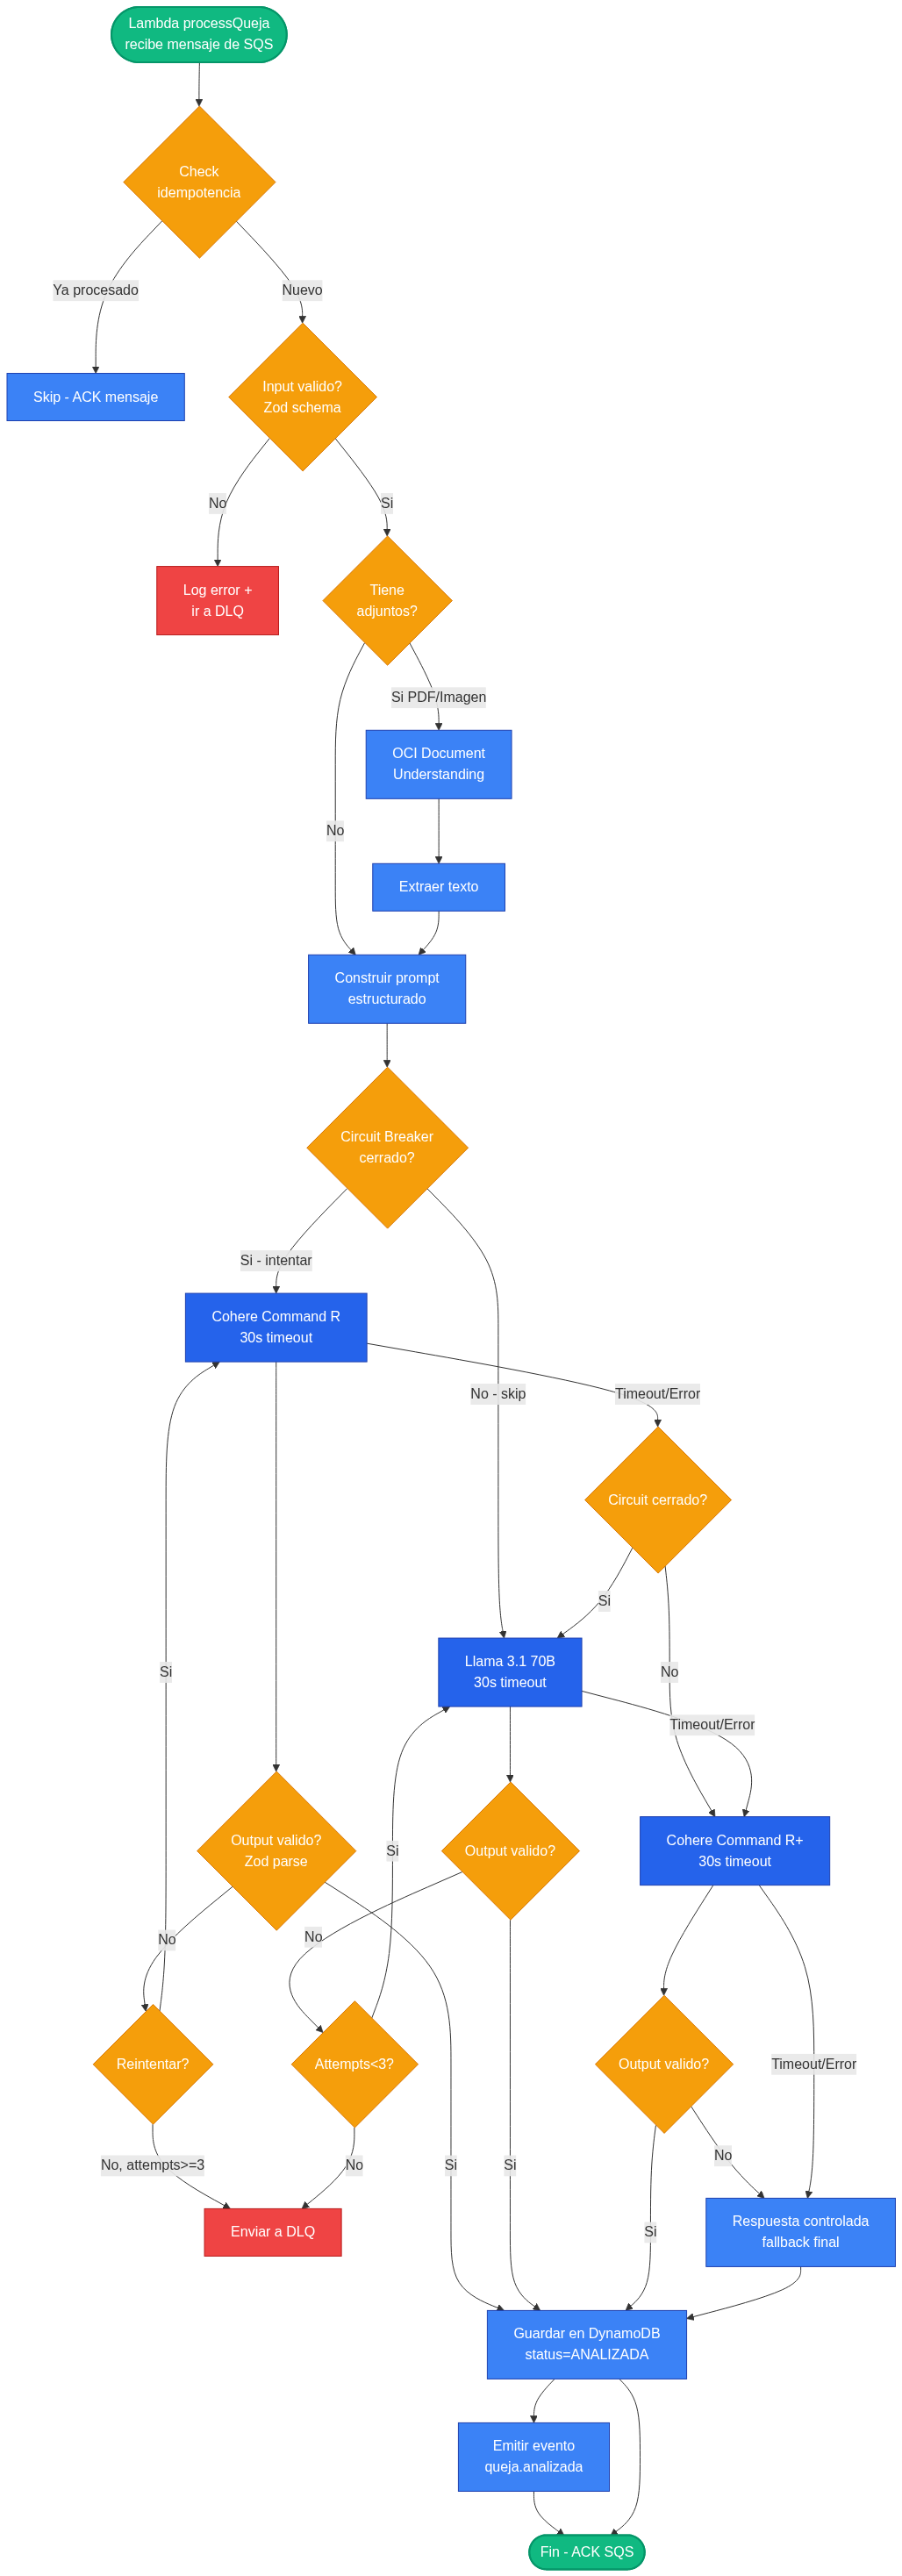
\includegraphics[width=0.95\textwidth]{diagrams/flujo-resiliencia.png}
\caption{Flujo completo de resiliencia en processQueja: idempotencia, validaci\'on, fallback chain entre 3 modelos LLM, circuit breaker, y degradaci\'on elegante a respuesta controlada.}
\label{fig:flujo-resiliencia}
\end{figure}

% ============================================
\section{Resultados Esperados y SLAs}
% ============================================

\subsection{SLAs objetivo}

\begin{longtable}{|p{5cm}|p{4cm}|p{4cm}|}
\hline
\rowcolor{primary!20}
\textbf{M\'etrica} & \textbf{Objetivo} & \textbf{Medici\'on} \\
\hline
\endhead
Tasa de \'exito en procesamiento & $\geq$ 99\% & CloudWatch Metric: ProcessSuccess / ProcessTotal \\
\hline
Tiempo de procesamiento (p95) & $<$ 30s & CloudWatch Metric: ProcessingDuration \\
\hline
Latencia del LLM (p95) & $<$ 20s & Custom Metric: LlmLatency \\
\hline
Disponibilidad del sistema & $\geq$ 99.5\% & CloudWatch Synthetics Canary \\
\hline
Detecci\'on de caso cr\'itico & $<$ 60s end-to-end & Tiempo entre POST /quejas y SNS publish \\
\hline
Tasa de falsos positivos (criticidad CRITICA) & $<$ 10\% & An\'alisis manual semanal \\
\hline
DLQ vac\'ia & 100\% del tiempo & CloudWatch Alarm \\
\hline
Circuit breaker cerrado & $\geq$ 95\% del tiempo & Custom Metric: CircuitState \\
\hline
\end{longtable}

\subsection{Cumplimiento de la r\'ubrica}

\begin{itemize}[leftmargin=*]
    \item \textbf{Circuit breaker en TODA llamada a LLM}: opossum configurado por modelo
    \item \textbf{Fallback entre 2+ modelos}: cadena de 3 modelos + respuesta controlada
    \item \textbf{Rate limiting}: token bucket por usuario e IP
    \item \textbf{Retry con exponential backoff}: p-retry con jitter
    \item \textbf{DLQ en TODA cola SQS}: redrive policy + alarma
    \item \textbf{Idempotencia en consumers}: SHA-256 + conditional writes en DynamoDB
    \item \textbf{Timeouts en TODA llamada externa}: configurados por servicio
    \item \textbf{Logging estructurado con correlationId}: propagado end-to-end
    \item \textbf{Prompt estructurado con validaci\'on Zod}: schema estricto + safeParse
    \item \textbf{Monitoreo}: CloudWatch + X-Ray + Langfuse + alarms
\end{itemize}

\vspace{0.5cm}

\begin{center}
\textit{``La resiliencia no es un lujo, es un requisito.\\Especialmente cuando se trata de bienestar de personas.''}
\end{center}

\end{document}
